\documentclass{article}

\usepackage{geometry}
\usepackage{listings}
\geometry{a4paper, margin=1in}
\usepackage{amsmath}
\usepackage{graphicx}
\usepackage[toc,page]{appendix}
\usepackage{caption}
\usepackage{subcaption}
\graphicspath{{./}}
\title{\textbf{Intro to Computer Vision \\Range Image Segmentation \\Lab-8}\vfill{}}

\author{\textbf{Submitted By:}\\Saroj Kumar Dash}

\begin{document}
	\begin{titlepage}
		\maketitle
		\pagenumbering{gobble}
	\end{titlepage}
	
\newpage	

\pagenumbering{arabic}
\textsl{•}\section{Introduction}
\paragraph{Range Image Segmentation}
In this project I segmented a range image based upon surface normals. I took the range image of a chair which was given at the course website. I also used some C-code that was also provided to convert the pixels into 3D coordinates. My segmentation process used the image grid for grouping pixels, but I used the 3D coordinates for calculating surface normals for my region predicates condition inside the region-grow function.

\section{Method and Results}
To get a good thersholding value I tried to find out a good imaging too; in my case irfan view to see the pixel values and to get a good threshold range values for pixels such that all of the floors of the image is retained.  \paragraph{Thresholding:}
The image was masked by thresholding at a distance that removes the background and leaves only the floor and the chair. The image was thersholded to below values.

Threshold range : Threshold Min = 20 , Threshold max = 120
\begin{lstlisting}
My Code: thresholdImage(tmpImg,20,120);
\end{lstlisting}


\paragraph{2d to 3d Coordinates}
Used the provided C-code to calculate 3D coordinates for the pixels. The slant type given in the scandirection downward.

My 3d Coordinates for the point(r,c)=108,87 is 14.682011,-28.632906,75.422777

\paragraph{region growing and results}
After that I found the cross product to find the surface normals to the surfaces and stored it in an array and then did the region growing by getting the avg normal and then finding angles to it.

\subsection{Results}
In my project I found 5 regions. Again the background or the wall is another region. Thus there are 6 regions detected. Below is the gray scale image of the result segmented image in my case:

Threshold for Normal angle predicate in degree = 51
The distance to take corss Product = 4

\begin{figure}[!htb]
    \centering
  		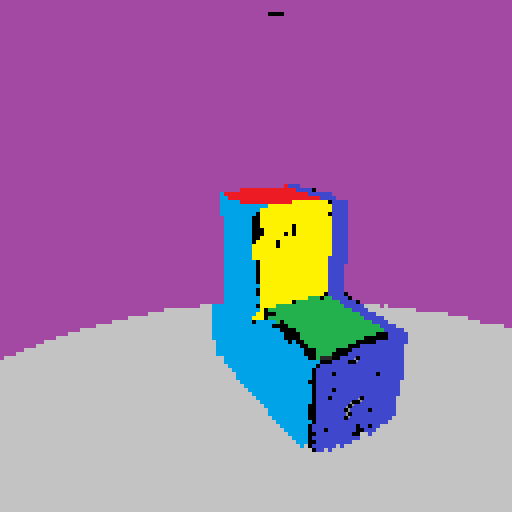
\includegraphics[scale=1]{outdeg_51_4.png}
  		\caption{Output image after segmentation of the gray scale range image, I got this output using mspaint so noot very accurate to show segments}
  		\label{Fig1}
\end{figure}

\begin{figure}[!htb]
    \centering
  		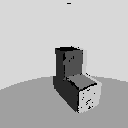
\includegraphics[scale=2.0]{outdeg_51_4bw.png}
  		\caption{Output image after segmentation of the gray scale range image in grayscale}
  		\label{Fig2}
\end{figure}
\newpage
I found 6 regions by my implemented range image segmentation algorithm. Below are the regions. So in total there 7, which is 6 my segments and 1 more from the thresholding of the image in which I set the background wall as a color 0 so it becomes a segment too. The segments which are colored in the image. 

\begin{enumerate}
\item{Region 1}
My region 1 segment is in black in my grayscale image .The top part of the chair which got submerged with background in case of the color image.

\begin{lstlisting}
\#pixels: Region labeled 1 is 713 in size;
pixel Value: 40;
Average Normal: (x,y,z) = (-22.522771,-1.136282,-8.195585);
\end{lstlisting}

\item{Region 2}
My region 2 segment is in dark grey in my grayscale image and in blue in the colored image. The left part of the chair.

\begin{lstlisting}
\#pixels: Region labeled 2 is 440 in size;
pixel value: 80;
Average Normal: (x,y,z) = (4.599245,-3.734720,-7.943015);
\end{lstlisting}


\item{Region 3}
My region 3 segment is in grey in my grayscale image and is in green color in the colored image. The back of the chair and the bottom of the chair was selected as the segments. I was expecting they will be of different segments but since the normals are parallel to each other and since they will be making same angle with avg surface normals so they got segmented together.

\begin{lstlisting}
\#pixels: Region labeled 3 is 235 in size;
pixel value: 120;
Average Normal: (x,y,z) = (-1.244708,14.551283,-4.527213);
\end{lstlisting}

\item{Region 4} 
My region 4 segment is the floor in my grayscale image and in gray in the colored image. 
\begin{lstlisting}
\#pixels: Region labeled 4 is 4932 in size
pixel Value set: 160
Average Normal: (x,y,z) = (-1.062503,13.862880,-4.779944)
\end{lstlisting}
\item{Region 5} 
My region 2 segment is in light grey in my grayscale image and in orange in the colored image. The seat of the chair.

\begin{lstlisting}
\#pixels: Region labeled 5 is 607 in size
pixel Value set: 200
Average Normal: (x,y,z) = (65.651862,-2.739392,-22.457364)
\end{lstlisting}


\item{Region 6} 
My region 2 segment is in white color in my grayscale image and in red color in the colored image. This part of the image was excluded to be segmented as we had already segmented it using thresholding.

\begin{lstlisting}
\#pixels: Region labeled 6 is 9224 in size
pixel value: 255
avg normal not available. As we did not need any procedure to segment this.
\end{lstlisting}

\end{enumerate}


\begin{figure}[h]
\begin{center}$
\begin{array}{llll}
\includegraphics[width=50mm]{../Final/region1_0.png}&
\includegraphics[width=50mm]{../Final/region2_40.png}&
\includegraphics[width=50mm]{../Final/region3_80.png}
\end{array}$
\end{center}

\begin{center}$
\begin{array}{rrrr}
\includegraphics[width=50mm]{../Final/region4_120.png}&
\includegraphics[width=50mm]{../Final/regioon5_160.png}&
\includegraphics[width=50mm]{../Final/region6_200.png}


\end{array}$
\end{center}
\caption{All the regions detected only the first region is regioon 1 and gves me black normals}
\label{pics:regions}
\end{figure}


\section{Conclusion}
So in total I was extract 5 surfaces from the image and the could segment it based on the normals. The results were not perfect but my algorithm rcognized nearly all the surfaces in the image.
\newpage

\section{Appendix}
\lstinputlisting[language=C++]{"../../letters.cpp"}
\label{appendix: Appendix A}


\end{document}